\chapter{Introduction}

In this dissertation, we optimize distributed computing workflows on a campus grid.  We are interested in optimizing a researcher's use of the computational and storage resources on the campus to increase the reliability and decrease the time to solution for scientific results.  We first extend prior work to enhance the computational capabilities of researchers on a campus.  We then expand our work to the data needs of modern workflows.

\section{Campus Grid Computing}

The increase of performance of computer hardware following Moore's law \cite{schaller1997moore} has allowed scientists to tackle larger problems.  As they increase their use of research computing, their applications far exceed the locally available resources.  Such applications often turn to distributed computing to aggregate more computational, memory, or storage resources than locally available resources can provide.

%Despite the ever increasing performance of computer hardware following Moore's law \cite{schaller1997moore}, applications continue to keep pace with hardware's capabilities as researchers tackle larger problems.  For some users, their applications far exceed the capabilities of computers that are immediately available to them.  Such applications may be able to use multiple computers to aggregate  more computational, memory, or storage resources than a single computer can \mbox{provide}.

Batch computing can combine the computational, memory, and storage resources of multiple computers in a single cluster through concurrent scheduling of applications.  A computational grid is an extension of batch computing, where resources may be combined from multiple pools of resources to be used for an application.

A computational grid is a hardware and software infrastructure that provides dependable, consistent, pervasive, and inexpensive access to high-end computational capabilities \cite{foster2004grid}.  A campus grid is a specialized grid where multiple resources are owned by the same organization, although it may be in multiple administrative domains.  
%For our discussion of computation, we restrict our consideration to those campuses that have multiple computational resources.

A campus grid has become necessary to spread demand across multiple clusters.  This is important when demand for a single cluster is large, due to improved performance or increased storage, and demand is low on other available clusters.  One aim for a campus grid is to move computation from the in-demand cluster to other clusters, which can result in a shorter time to completion for the users' jobs.

To succeed, a campus grid requires a framework to distribute jobs to multiple clusters in a campus.  In \cite{weitzel2011campus}, I proposed a solution based on HTCondor \cite{litzkow1988condor}.  The solution required installation of a campus factory \cite{website:campusfactory} on each cluster's login node.  An on-demand overlay was created that could efficiently run high throughput jobs on multiple campus resources.  

Although my solution was efficient and fault tolerant, it was deficient in several ways.  Installation and setup of the campus factory was difficult since it was not automated.  The communication inside the overlay was insecure.  We set out to correct these deficiencies.

%Users had to install HTCondor on both the cluster's login node and the user's submit node.  Also, the security setup was based on IP whitelists, which can be defeated with IP spoofing.  Therefore, we set out to correct these deficiencies.

We have enhanced my Masters thesis' solution to include:
\begin{itemize}
\item Easier installation through automation
\item Increased security through secure key exchange
\item More supported cluster types and configurations
\item Improved access to computing through language frameworks such as R \cite{team2005r}
\end{itemize}

We created a framework for job submission to remote resources that the user does not control.  Typical grid submission uses custom interfaces such as the Globus Resource Allocation Manager (GRAM) \cite{foster1999globus}, which is previously installed by an administrator.  We assume resources do not have such dedicated grid software installed.  This framework does not require administrator intervention for remote submission to opportunistic resources.  The framework uses interfaces that are installed on nearly all clusters that are typically used for interactive access.  It automates the submission and error handling of jobs submitted to remote resources, while providing the user a consistent interface over multiple, load-balanced clusters.

The new framework is named Bosco \cite{weitzel2014accessing}.  It uses secure protocols to connect to remote clusters in order to transfer files and submit/monitor jobs.  Installation of Bosco on remote clusters and the submit host has been automated with simple tools.  Clusters with restrictive firewalls are supported by multiplexing operations through a single secure connection.  Furthermore, many cluster schedulers are supported by the underlying technology.  A diagram of the architecture of Bosco is shown in Figure \ref{fig:introboscoarch}.

\begin{figure}[h!t]
	\centering
	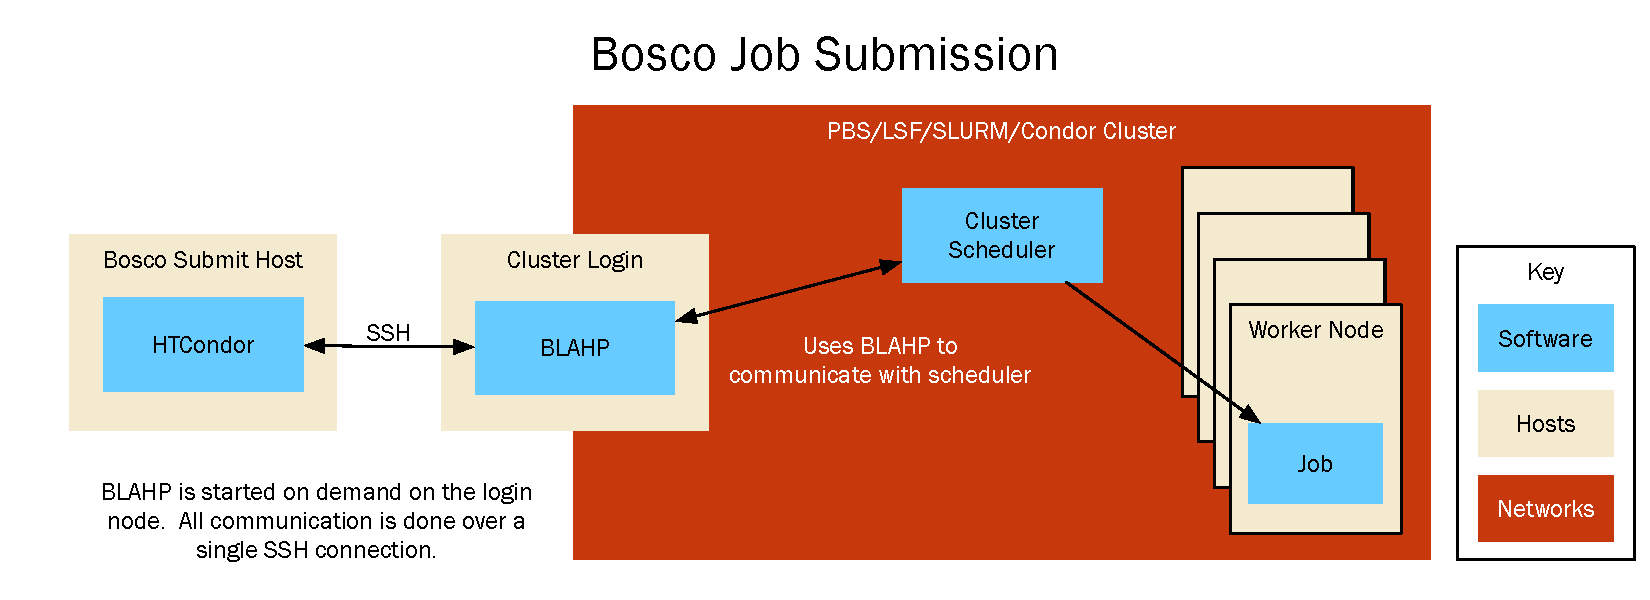
\includegraphics[width=\textwidth]{images/ArchitectureGraph1.pdf}
	\caption{Bosco Architecture}
	\label{fig:introboscoarch}
\end{figure}

Bosco, in coordination with technologies in HTCondor, enable a job distribution method which is provisioned based on demand.  A default Bosco installation is able to submit to one local cluster.  If that cluster does not meet the user's computational needs, then Bosco can be configured to submit to multiple clusters with load balancing between them.  If the user's computational needs are still not met with multiple clusters, they can configure Bosco to submit resource requests to national cyberinfrastructure such as the Open Science Grid (OSG) \cite{pordes2007open}.  The provisioning capabilities of Bosco creates an ever expanding network of available resources. The goal is to provide an expanding network of resources as shown in Figure \ref{fig:boscogrowing}.

\begin{figure}[h!t]
	\centering
	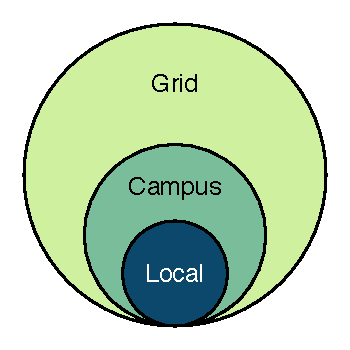
\includegraphics{images/BoscoGrowing.pdf}
	\caption{Bosco's Growing Reach as Demand Increases}
	\label{fig:boscogrowing}
\end{figure}

In order to ease access to Bosco for data processing, an interface has been developed in the most widely used data processing language, R.  This BoscoR framework enables users to never leave their R environment in order start remote data processing.

But Bosco is not enough for researchers that have large data requirements.  Input and output data are explicitly listed by the user.  The data is transferred over the secure, but slow, connection between the submitter and resource for every job.  Therefore, we must consider data and storage management on the campus grid.


%Most major research campuses, whether a university campus, or a national lab campus, have a research computing resource.  The computing resources are broken into two categories:

%\begin{itemize}

%\item Condominium - Resources are purchased by research groups for their dedicated use.  They are added to a cluster that may share infrastructure such as a filesystem or an interconnect.
%\item Shared resources -  Resources are purchased by a central authority that are shared between multiple research groups.

%\end{itemize}





\section{Data Management on Campus}

There are many challenges in data management and distribution in scientific computing \cite{deelman2008data}.  For batch computing, one challenge is transferring the data from the user's computer to the execution resources.  Large data workflows can strain the network near the data's source, which can result in unreasonable amounts of batch time used solely for data transfer.

Data management is the framework and policies controlling data through the research cycle.  In this dissertation, we are concerned with optimizing data management when using campus computational resources.

As users spread their computation across multiple clusters either on the campus or across campuses, data distribution and collection becomes more difficult.  Before using the campus grid, a user would select a cluster to do their processing.  The user then could host all of their data on that cluster by copying the data onto that cluster's shared filesystem.  The jobs access the data from the shared filesystem just as it would on the user's desktop, available for all executions at the same directory.

These assumptions do not hold for a campus grid.  A grid is made up of multiple computational clusters, with potentially many separate filesystems; no single filesystem is accessible access from every computational resource.  Further, the shared filesystem could become a bottleneck if many jobs are requesting the same data simultaneously.  Therefore, data management techniques must evolve along with computation.  


Most distributed batch schedulers are able to transfer the input data for each job execution.  Each job starts with an empty execution area and the scheduler will transfer the files into it.  When the user is not using the scheduler to transfer data, the input data must still reach the execution host.  Data will be transferred from the source (usually the user's computer) to the execution resources for processing.  The network connection between the source and the execution resources may be a bottleneck for the computation.  Frequent re-transfers of the same input data will further congest the network between the source and the execution resources.

In this dissertation, we optimized two attributes of distributed data management: efficient transfer methods and reduction of duplicate transfers.

We introduce the CacheD \cite{weitzel2015pdpta}, a caching and data transfer daemon for input data in distributed computing.  The CacheD uses novel data management methods based on technology developed for large peer-to-peer data transfers on the Internet, BitTorrent.  It also caches input data on the execution resources to enable quick transfers on subsequent requests for the same input data.

Similar to the work with Bosco, the CacheD does not require privileged access in order to provision storage resources.  It can use the storage on worker nodes spread across multiple clusters as a data input caching system.

\section{Data Distribution Policy Language}

Users of grid submission software currently have to describe how their files will be transferred from their submission host to the remote execution resource where the data will be processed.  They have to coordinate the storage and computational resources without help.  We propose a policy language that allows an agent to decide an appropriate method for data transfer.  It determines the transfer method by negotiating between the following three sources: a user-given policy language for the data, the remote execution resource's capabilities and preferences, and the submitting resource's capabilities and preferences.  In addition, the policy language should determine if the cache should be replicated to multiple resources.  A modern flexible policy language for describing data distribution for campus users is needed.

In addition to the CacheD described above, a policy language must be made in order to help the CacheD make decisions when interacting with other agents, such as other CacheDs or the local node.  We discuss extending this policy language to include custom attributes that users can include to improve choices on data distribution.

The policy language utilizes the \mbox{ClassAds} \cite{raman1998matchmaking} language.  These \mbox{ClassAds} were originally developed in the context of matchmaking between computational resources and potential jobs.  ClassAds are a schema-free language for describing heterogeneous resources.  We demonstrate usage with new attributes that pertain to storage and expressions that can be evaluated to make decisions.

The user must specify preferences for the cache to consider.  Examples include: where should this cache be distributed, how should the cache be distributed, and how long the cache should be stored.  Each of these preferences must be negotiated with the preferences of the CacheD that may store or is storing the cache.  The user's preferences will affect how fast the cache is transferred (different transfer methods are more efficient than others) and also, on which and how many nodes that cache should be replicated.

Further, each CacheD must coordinate with one another in order to distribute the caches in an efficient method.  Replication of caches between CacheDs must be negotiated.  A CacheD may decide, through evaluating its own policies, whether or not to accept a cache to be stored.  These policies are again expressed in the ClassAd policy language.



\section{Overview of Dissertation}

This dissertation describes how data intensive applications can be run in a distributed campus environment.

\begin{description}
	\item[Chapter \ref{chapter:relatedwork}:]  There are many distributed computing platforms available publicly.  In this chapter, we will discuss these schedulers and differentiate them with Bosco.  Also, we will discuss other available data management, distributed storage, and caching systems.
	
	\item[Chapter \ref{chapter:campusjobs}:] We will discuss how computing can be managed on the campus using the Bosco framework.  We will also discuss a case study of integrating Bosco with the programming language, R, in order to provide an easy-to-use interface to campus distributed computing.
	
	\item[Chapter \ref{chapter:campusdatadistribution}:] We will discuss the CacheD, a campus data distribution service.  The CacheD is able to combine novel transfer methods with data caching to improve the stage-in time for large data sets.  Through evaluation, we show that the CacheD demonstrates a significantly shorter stage-in time for large data sets over existing solutions that have been deployed.
	
	\item[Chapter \ref{chapter:campusstoragepolicylanguage}:]  
	Simply caching and transferring data does not provide the flexibility that the CacheD requires to operate in a distributed environment.  In this chapter, we will discuss the policy framework and language that enable the CacheD to interact with the user and other daemons in order to make decisions.
\end{description}


\newpage
\section{A Note on Terms}
High performance and distributed computing often use terms inconsistently.  Below is a definition list of such terms, and how we will define them for this dissertation:


\begin{description}
	\item[Job:] A packaged unit of work with input and output.  A job may consume computational, memory, network, and/or storage resources in a batch system.
	\item[Workflow:] A logical grouping of jobs executed on resources.  The jobs may have some ordering.
	\item[Campus:] An organization that may have multiple administrative domains which may vary access policies to resources.
	\item[Execution Resource:] A resource which fulfills the requirements of a job and may also run it.  This may be a worker node in a cluster.
	\item[Cluster:] A set of execution resources that have high interconnection bandwidth and are managed by a single scheduler.
	\item[Batch System:] A scheduler for the resources of a cluster.
	\item[Agent:] An independent entity that can make decisions on its own without the control of another entity.  In this dissertation, we will use the word agent to describe a daemon which can make independent decisions without the explicit control of other daemons.
	\item[Pilot:] Pilot jobs are containers that once started, will request work from the user's job queue.
\end{description}



